\section{Classifiers}

\subsection{Implementation}

\subsubsection{Mean Euclidean Distance}

The MED classifier uses the class means as prototypes for the classifier. The class membership is determined by specifying the class which has the smallest euclidian distance from the class mean to the test point.

\subsubsection{General Euclidean Distance}
The GED classifier is implemented in a similar manner as the MED classifier. However, in the case of GED a whitening transform is applied to the samples to transform them onto a space where features are both uncorrelated, and have unit-variances. This is accomplished using the weighting matrix W. The distance between two points in the transformed space is calculated as:


\begin{eqnarray}
\label{eqn:GED-whitening}
\left [ W=\Lambda^{-1/2}\Phi^{T}  \right ]
\end{eqnarray}



In the above equation, $\Lambda$ contains the eigen values of the covariance matrix $\Sigma$ as elements, and $\Phi$ contains the eigenvectors of $\Sigma$. The simplified distance function is included in Equation~\ref{eqn:GED}.

\begin{eqnarray}
\label{eqn:GED}
{d}_{G}(x,z) = {\left [ (x-z)^{T}\Phi\Lambda^{-1/2}\Phi^{T}(x-z) \right ]}^{1/2}
\end{eqnarray}


The decision boundary is therefore calculated in the two- and three- class cases as,

\begin{eqnarray}
\label{eqn:boundary-GED}
& d_{E} (x,z_{1}) = d_{E} (x,z_{2}) \\
& \left [ (x-{z}_{1})^{T}\Phi\Lambda^{-1/2}\Phi^{T}(x-z_{1}) \right ]^{1/2} \\
= & \left [ (x-z_{2})^{T}\Phi\Lambda^{-1/2}\Phi^{T}(x-z_{2}) \right ]^{1/2}  \nonumber \\
&\left [ (x-{z}_{1})^{T}\Phi\Lambda^{-1/2}\Phi^{T}(x-z_{1}) \right ]^{1/2} \\
= &\left [ (x-z_{2})^{T}\Phi\Lambda^{-1/2}\Phi^{T}(x-z_{2}) \right ]^{1/2}  \nonumber \\
= &\left [ (x-z_{3})^{T}\Phi\Lambda^{-1/2}\Phi^{T}(x-z_{3}) \right ]^{1/2}  \nonumber
\end{eqnarray}



In the case of the MATLAB implementation, all points on the grid are classified based on identifying the minimum distance between the point and the mean of each class in the transformed space. This allows for a simple contour to be plotted showing the decision boundary between each class. This is shown below for both the two- and three- class case,

\begin{eqnarray}
\label{eqn:pointClass-GED}
min(d_{E} (x,z_{1}), d_{E} (x,z_{2})) \\
min(d_{E} (x,z_{1}), d_{E} (x,z_{2}), d_{E} (x,z_{3}))
\end{eqnarray}


This implementation of the GED classifier and method for creating the decision boundary is shown in Appendix A.

\subsubsection{Maximum A Posteriori}

The MAP classifier was being used on known distributions, namely normal distributions. The likelyhood $p(\underbar{x} \mid Y)$; where $Y$ is a class among A,B,C,D,E; was calculated for each class at each point in the grid. The classifier then skewed the distributions according to the prior probabilities. Pairwise comparisons were made among the 3 class case in order to determine the class.

\begin{eqnarray}
\label{eqn:pointClass-MAP}
 max \left( p(\underbar{x} \mid A)p(A), \hspace{3mm} p(\underbar{x} \mid B)p(B) , \hspace{3mm} p(\underbar{x} \mid C)p(C) \right) 
\end{eqnarray}

\subsubsection{Nearest Neighbor}

The nearest neighbor classifier uses MATLAB implementation of $knnclassify$. A nearest neighbor classifier will test a point and compare its distance to all other known classified points. The test point will belong to the class which contains a point with the least Euclidian distance to the test point.

The classification boundary is constructed by evaluating many test points on a grid, using the generated data as training data. Due to the nature of nearest neighbor, all training data will be classified correctly; each classified point is its own nearest neighbor.

\subsubsection{Five Nearest Neighbor}

The 5NN classifier uses MATLAB implementation of $knnclassify$. A nearest neighbor classifier will test a point and compare its distance to all other known classified points. The 5 nearest classified points are determined, and the class of each of the points is determined. The class with the majority of class points in the 5 nearest neighbors is designated the class for the test point.

Note that the method of selecting the 5 nearest sample points from each class and selecting the class with the lowest sample mean was not used, as there exist many variations of the nearest neighbor method, and the MATLAB default is likely the default due to its accuracy.

The classification boundary is constructed by evaluating many test points on a grid, using the generated data as training data. Unlike nearest neighbor, 5 nearest neighbor will not classify all training data correctly; the use of 5 nearest neighbors means that not all points will have 2 other nearest neighbors that are of the same class.



\subsection{Results}
All classification methods were applied in each of Case 1 and Case 2. To aid in analysis, MED, GED, and MAP classifier boundaries are all plotted together in one figure, along with data clusters and unit standard deviation contours. In the Case 1 scenario (Figure~\ref{fig:med_ged_map_classifier_case1}), the GED and MAP classification boundaries, shown as magenta and blue lines respectively, lie on top of each other with the magenta line being obscured. This is because the MAP classifier is reduced to GED in this case, as the a priori probabilities for each class are equal. The classification boundaries are essentially two very slightly curved, but relatively straight, lines separating the two data clusters. The MED classification boundary is represented by the steeper straight cyan line. This makes sense intuitively, as the classification boundary represents the perpendicular bisector of the mean in each cluster. In the MED case only the mean, and not the covariance information for the two classes, is considered.

\begin{figure}[ht]
\centering
	{
	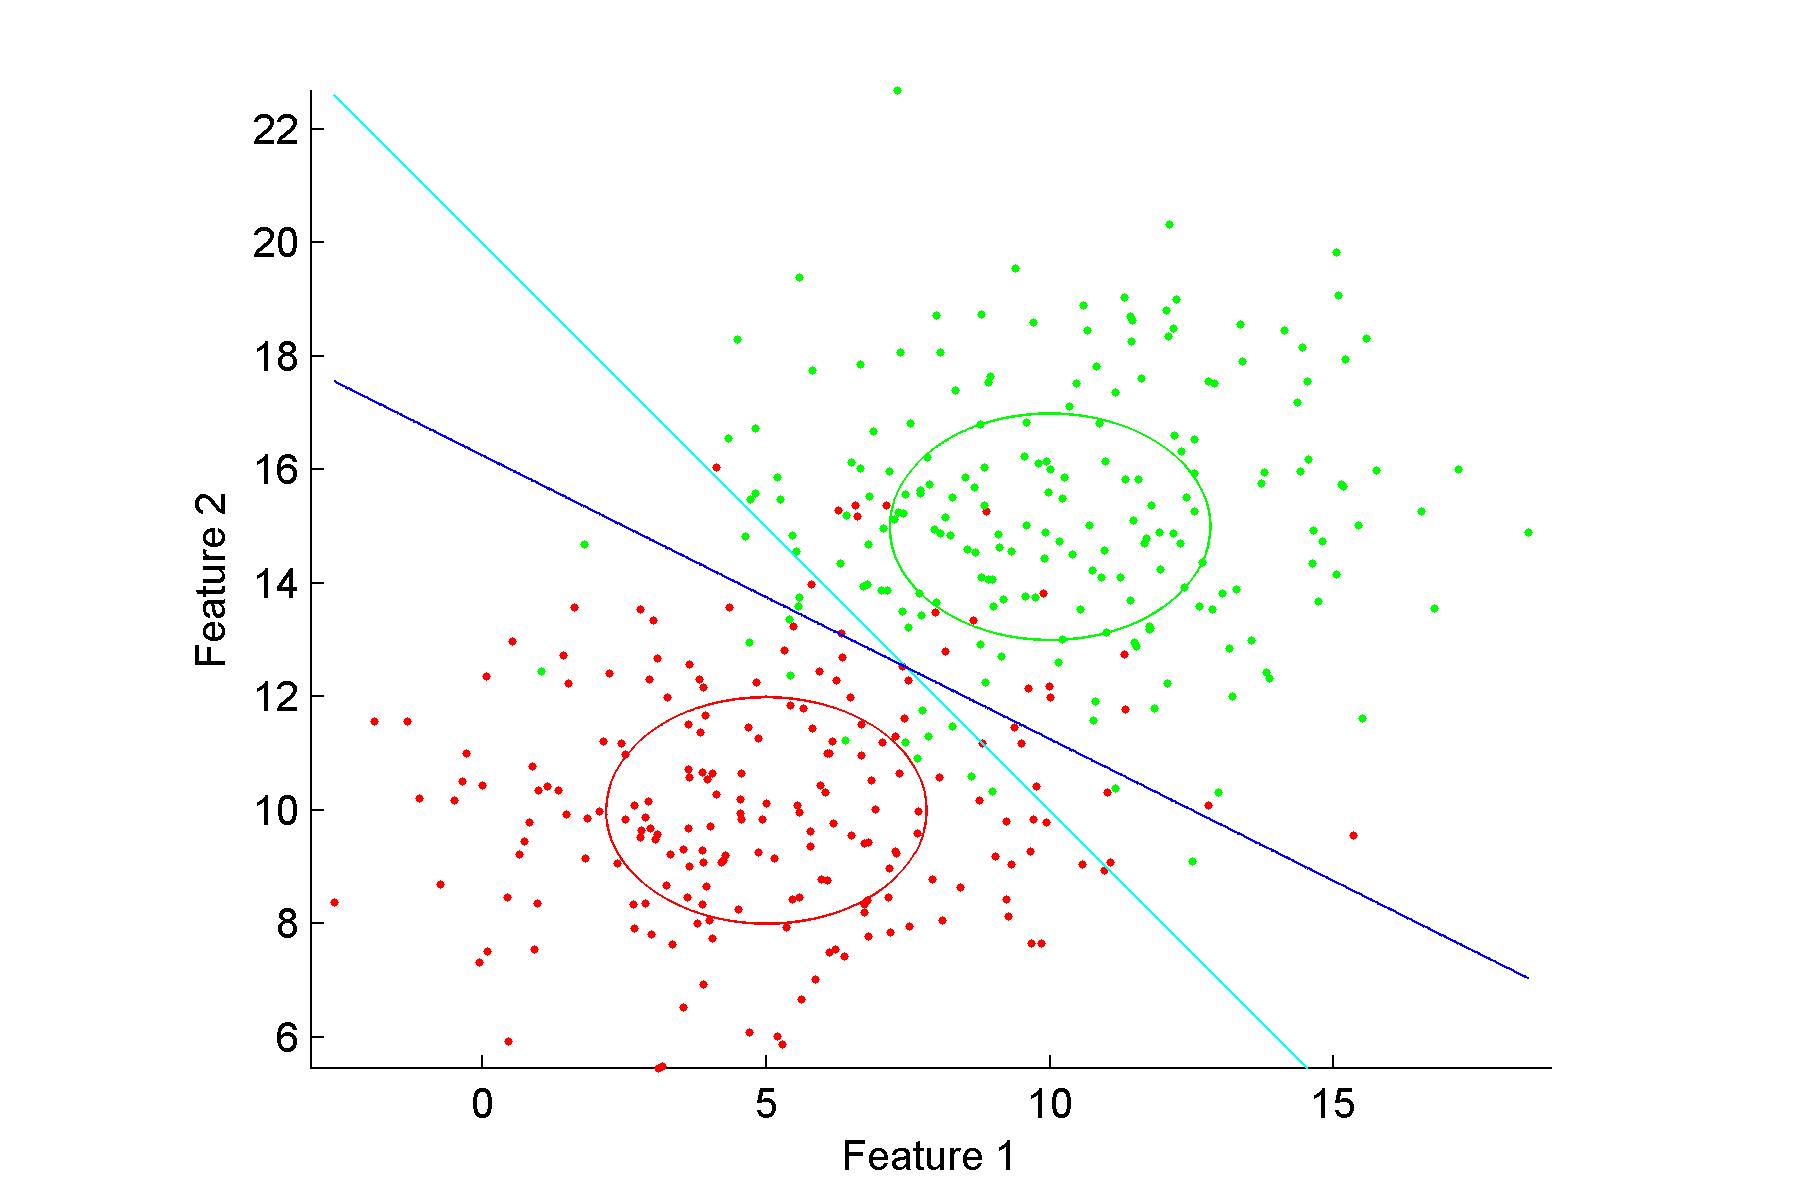
\includegraphics[width=0.45\linewidth]{fig2a-AB_MED_MICD_MAP}
	}
	
	\caption{MED, GED, and MAP classification boundaries for Case 1}
	\label{fig:med_ged_map_classifier_case1}
\end{figure}

In the Case 2 scenario (Figure~\ref{fig:med_ged_map_classifier_case2}), the MED classification boundary is shown as the light blue lines. The MED classification boundary is shown to be three straight lines, intersecting near the mid-point between the three data clusters. The MED classifier does not take into account the covariance matrices of the three data clusters, so the performance described is as expected. The GED classification boundary is shown as the contoured magenta lines in the figure, intersecting near the midpoint between the three classes of data. This is an intuitive result, as the classification boundary better wraps around the unit standard deviation contours for three data classes. The MAP decision boundary is shown as the blue lines, slightly offset to the left of the GED decision boundary. In this case the decision boundaries do not overlay each other as in the Case 1 scenario. This is a result of the a priori probabilities for each of the three classes being different in this case, with the probability information altering the performance of the classification method.

\begin{figure}[ht]
\centering
	{
	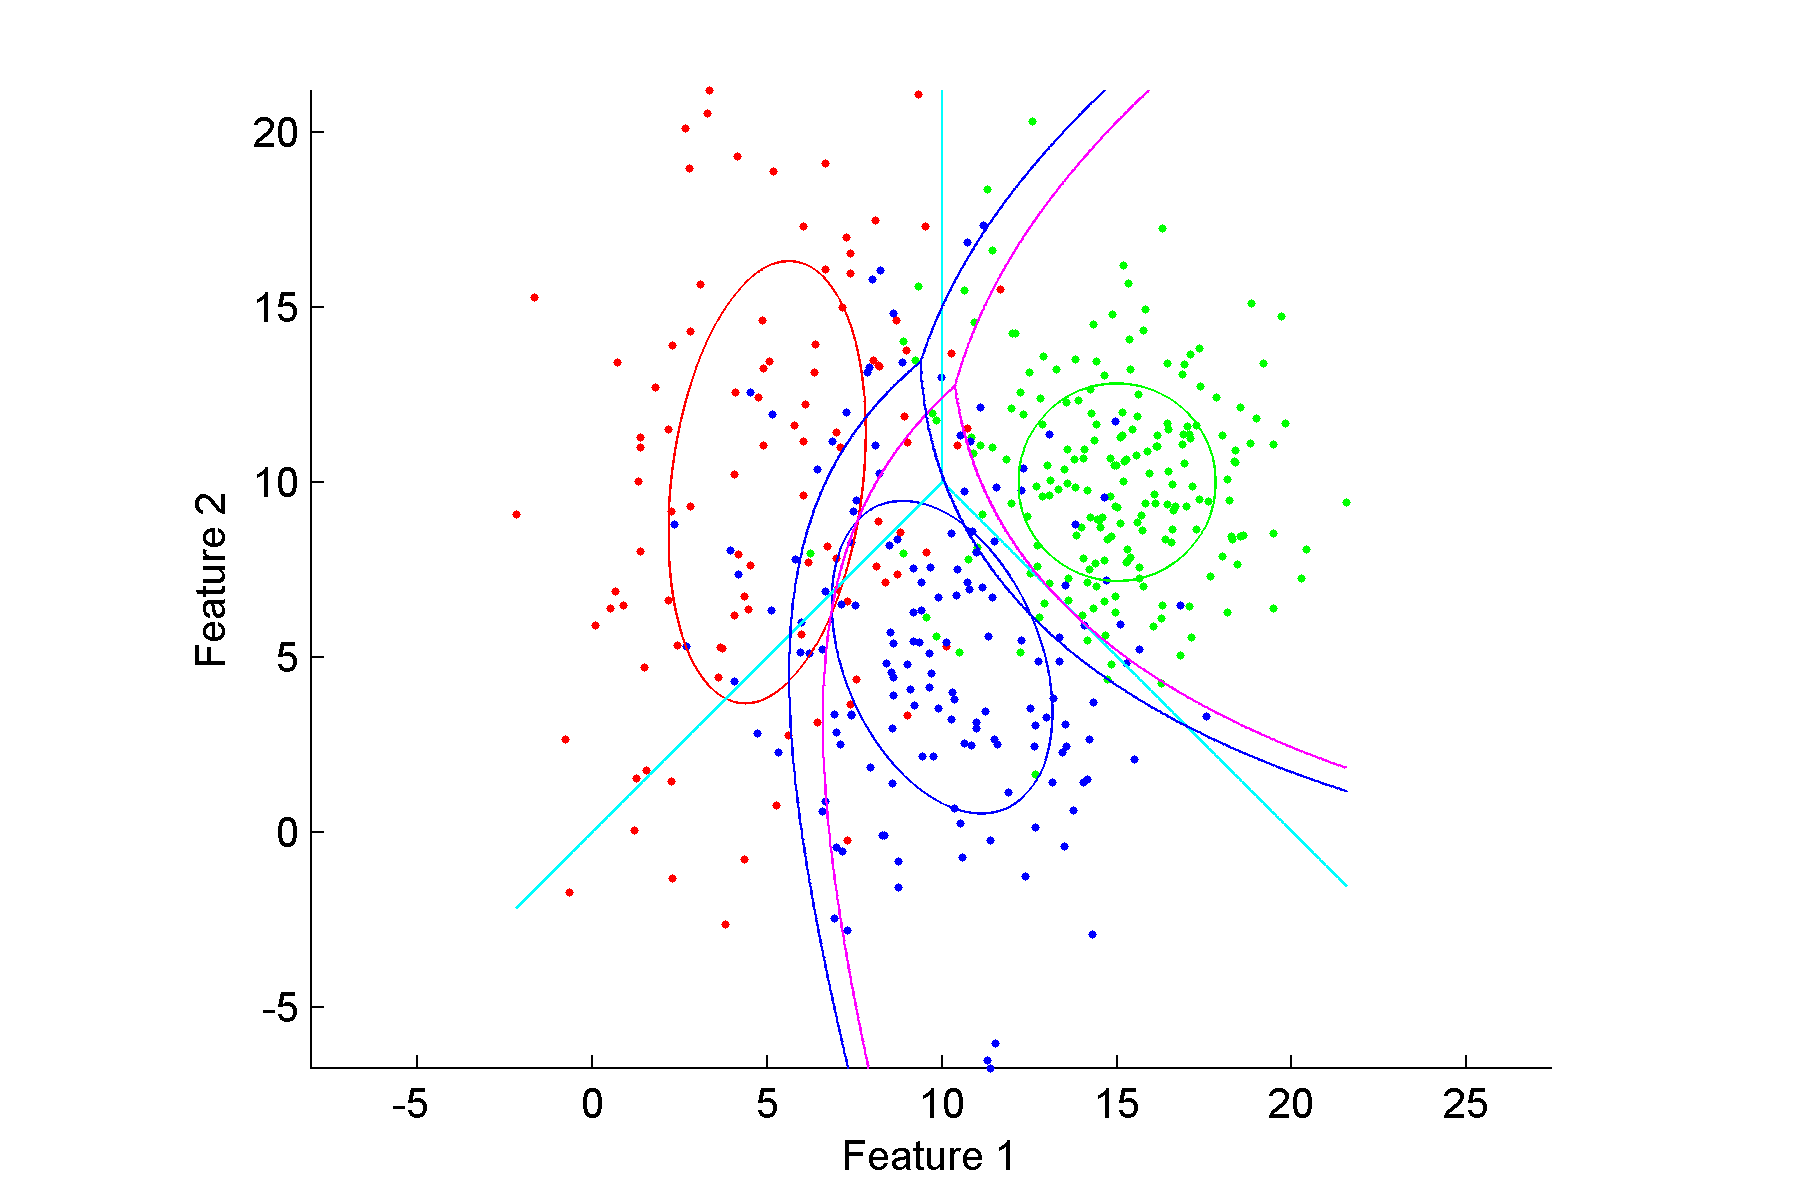
\includegraphics[width=0.45\linewidth]{fig2b-AB_MED_MICD_MAP}
	}
	
	\caption{MED, GED, and MAP classification boundaries for Case 2}
	\label{fig:med_ged_map_classifier_case2}
\end{figure}

Next, the NN and 5NN classification boundaries were plotted together for both the Case 1 and Case 2 data sets, along with unit variance contours for each class, to allow for comparison. The decision boundaries for Case 1, Figure~\ref{fig:nn_boundary_case1}, are fairly similar for both methods, with the decision boundaries being shown as jagged lines separating the data. The key difference in the two methods is that the 5NN classification method does not result in classification boundaries around outliers of the two data sets.

\begin{figure}[ht]
\centering
	\subfigure[NN classification for Case 1]{
	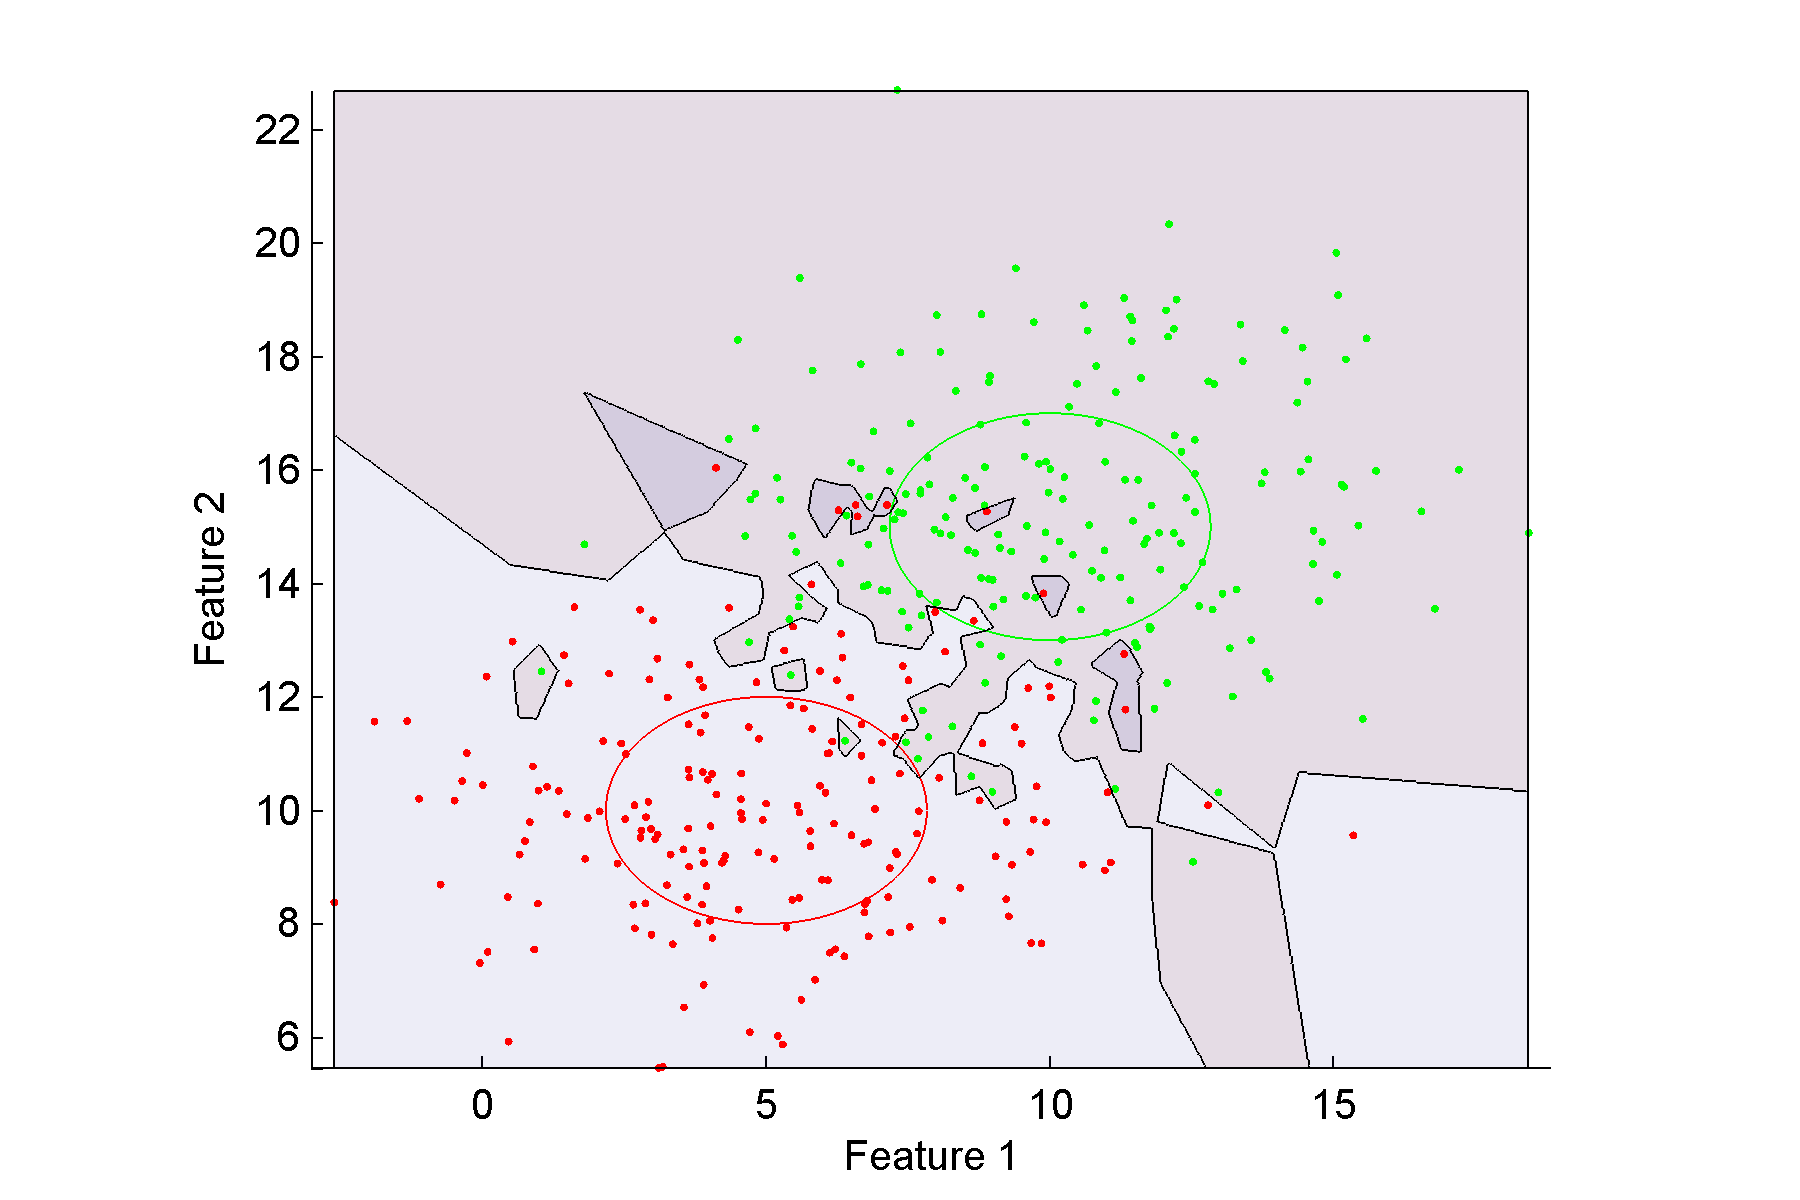
\includegraphics[width=0.45\linewidth]{fig3a-AB_NN}
	}
	\subfigure[5NN classification for Case 1]{
	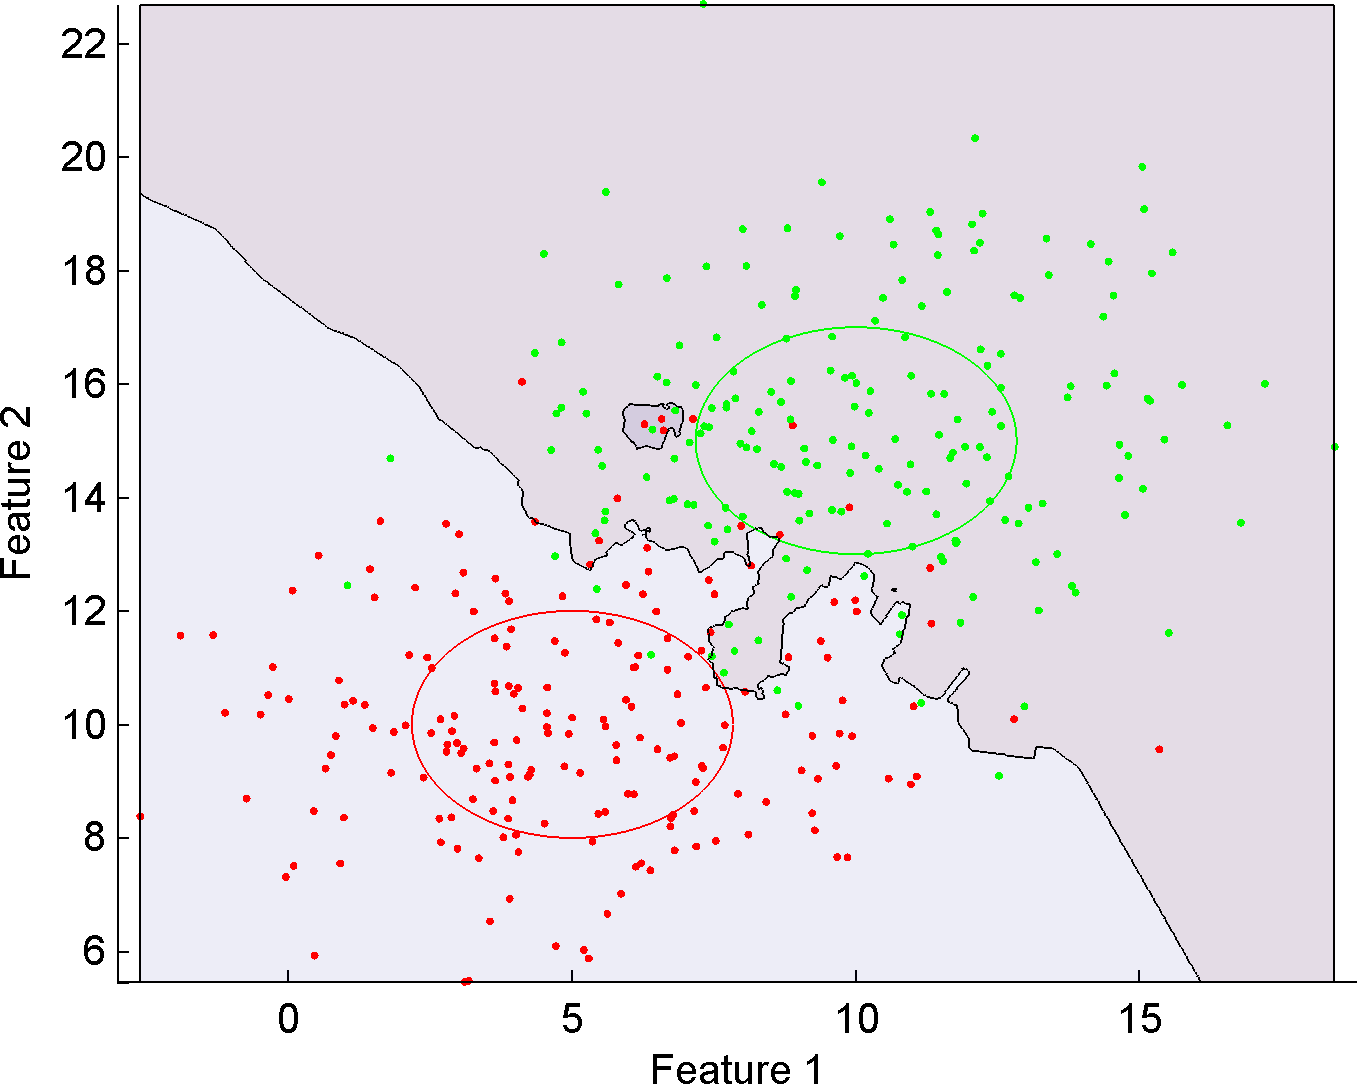
\includegraphics[width=0.45\linewidth]{fig4a-AB_5NN}
	}
	
	\caption{Nearest Neighbor boundaries for Case 1}
	\label{fig:nn_boundary_case1}
\end{figure}

For the Case 2 scenario, Figure~\ref{fig:nn_boundary_case2}, performance of the two methods was similar. Again, the sensitivity of the NN method to outliers is seen to result to decision boundaries encircling outliers. The 5NN classifier is not as prone to these outliers, resulting in a more intuitive decision boundary between the three classes of data.

\begin{figure}[ht]
\centering
	\subfigure[NN classification for Case 2]{
	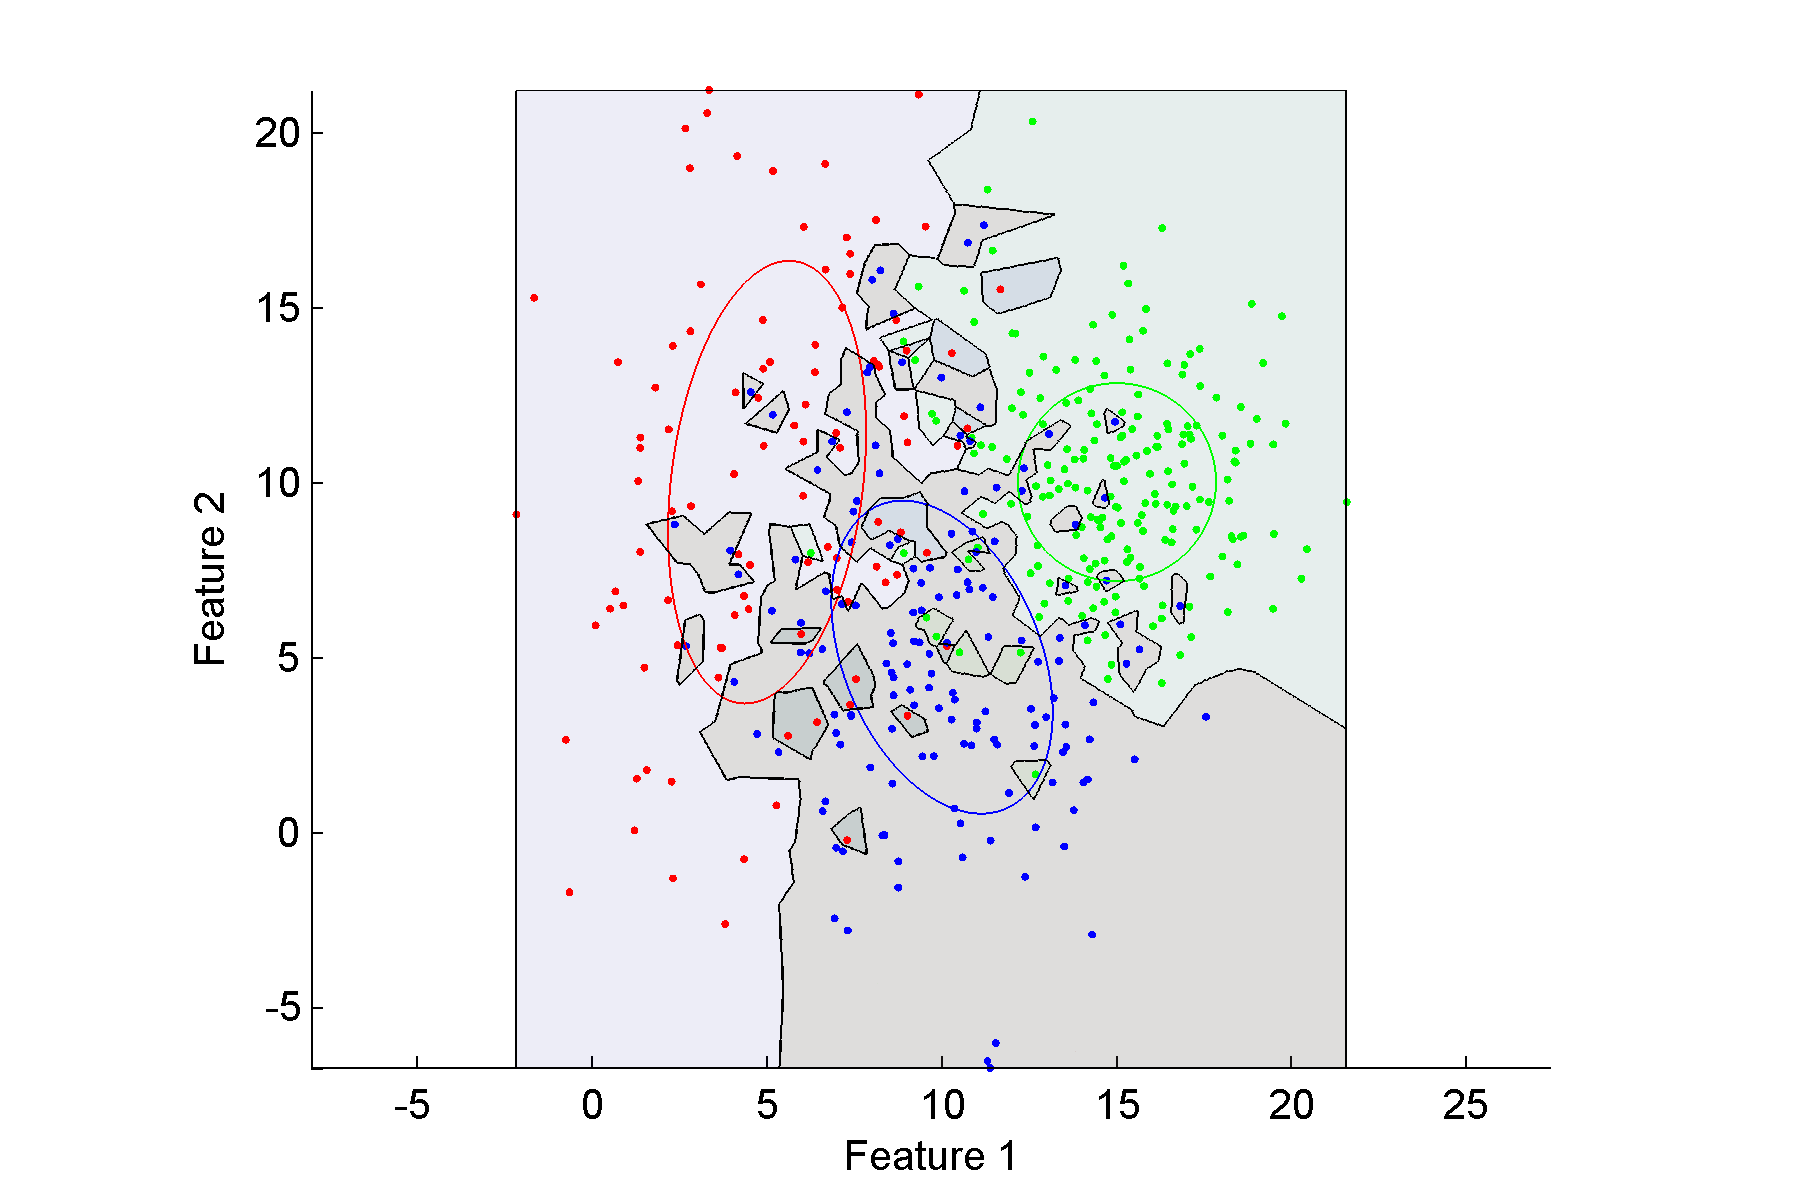
\includegraphics[width=0.45\linewidth]{fig3b-CDE_NN}
	}
	\subfigure[5NN classification for Case 2]{
	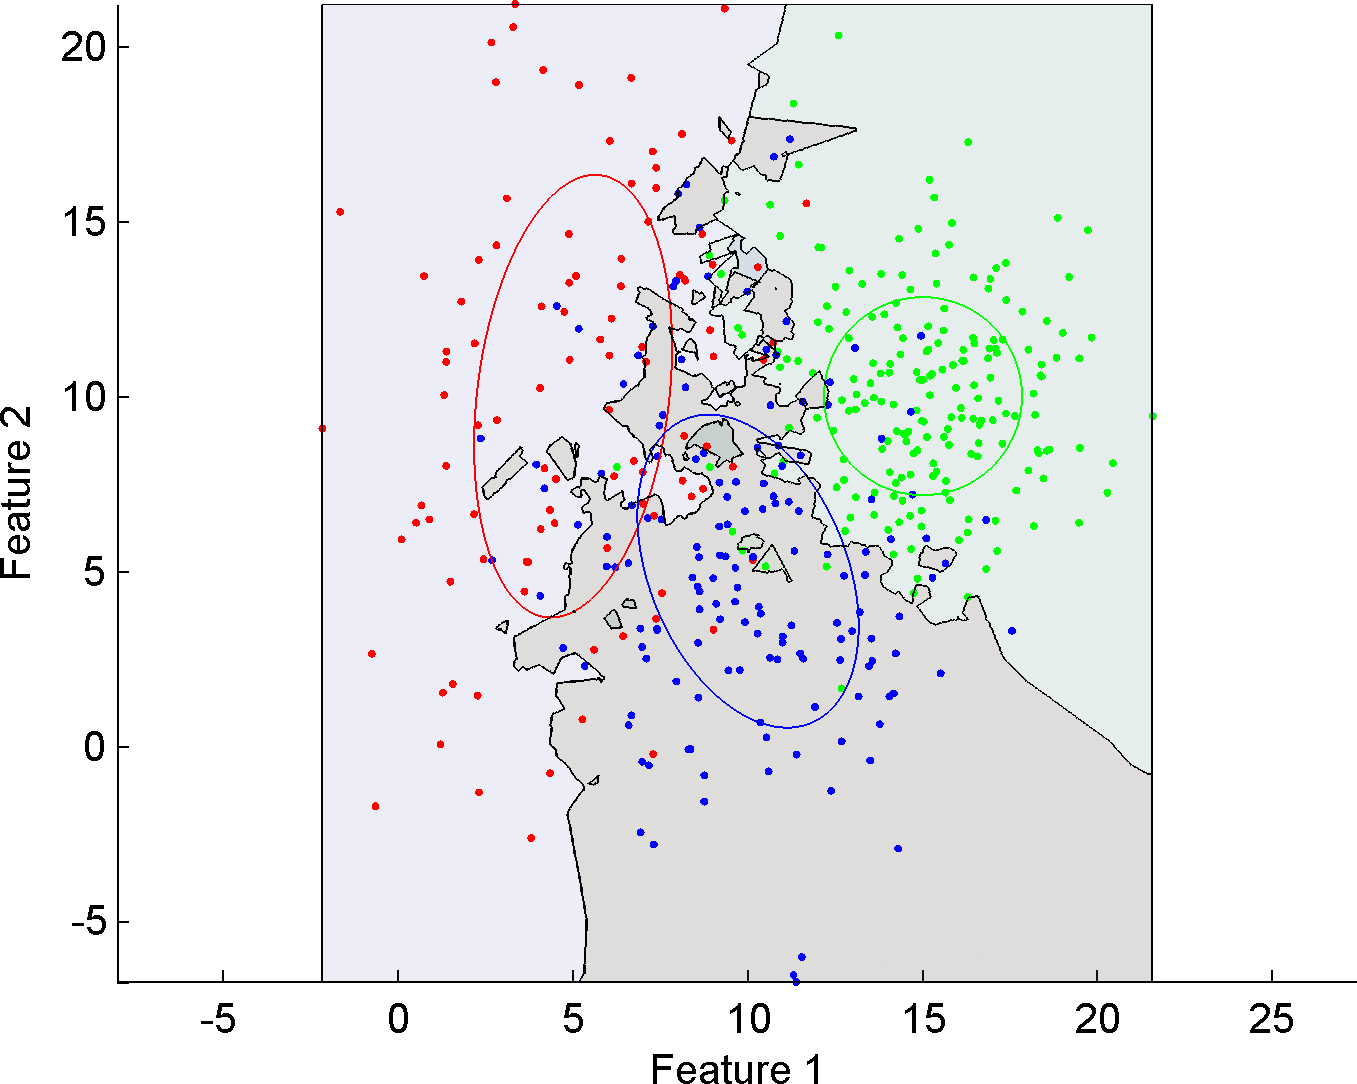
\includegraphics[width=0.45\linewidth]{fig4b-CDE_5NN}
	}
	
	\caption{Nearest Neighbor boundaries for Case 2}
	\label{fig:nn_boundary_case2}
\end{figure}
